\chapter{Coordinate Geometry}

\section{Introduction}
Many of you have encountered some form of coordinate geometry in high school. For instance, the "standard" way to visualize a graph e.g. $f(x)=x^2$ is to visualize the points in 2-D space $(x,y)$ where $y=x^2$. We give an demonstration in Python code.

\begin{lstlisting}[language=Python]
import matplotlib.pyplot as plt
import numpy as np
X=np.array(range(-100,100)) #create list of numbers from -100 to 100
Y= X**2 #calculate the square of at each x
plt.plot(X,Y) #plot all the pairs of points in 2d plane
plt.xlabel('x')
plt.ylabel('y=x^2')
plt.title('Visualization of the "object"')
plt.show()
plt.show()
\end{lstlisting}
\begin{tikzpicture}
	\node (A) at (0,0) {$x$};
	\node (B) at (3,0) {$x^2$};
	\draw[->,thick]
	(A)--(B)
	node[midway,below] {the "graph" object} ;
	\node(whitehead) at (8,0){
		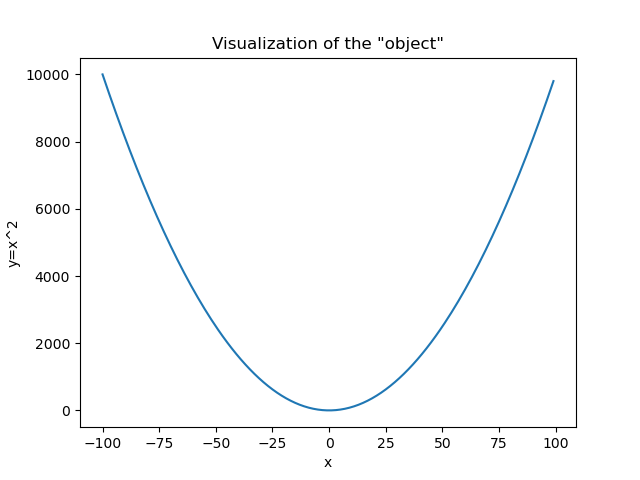
\includegraphics[width=0.6\textwidth]{coordinate_geometry/square_graph.png}
	};
\end{tikzpicture}


This is also known as the Cartesian plane, after Descartes who invented it in the 17th century.\\
\section{Visualization of geometric objects}
The Cartesian plane allows us to describe shapes with equations and perform calculations with them. We first define the playing field (the Cartesian plane and higher dimensional analogues) and the players.
\definition{Real numbers}{
	The set of \textbf{real numbers}, denoted as $\mathbb{R}$, is (informally) the set of all the numbers that can be written out in decimal form.
}
\example{
The following are real numbers:
\begin{enumerate}
	\item The integers $0$, $\pm 1$, $\pm 2$, ...  
	\item Fractions in the form $\frac{a}{b}$, where $a$ and $b\neq 0$ are integers.
	\item Irrational numbers $\sqrt{2}$, $\pi$.
\end{enumerate}
}
\begin{remark}
	The set of real numbers is known as a \textbf{complete field}. The definition of a complete field will be swept under the rug, but it guarantees a few things. The most important property: We will not "escape" the set by performing operations, possibly infinitely many.
\end{remark}
\definition{N-dimensional space}{
	Let $n$ be a positive integer. We denote the \textbf{n-dimensional real space} to be $\mathbb{R}^n$, consisting of all the $n$-tuples $(x_1,x_2,x_3,...,x_n)$, where each $x_j$ is a real number. \\
	We call an $n$-tuple $(x_1,...,x_n)$ a \textbf{point}, and two points $(x_1,...,x_n)$ and $(y_1,...,y_n)$ are equal if $x_j=y_j$ for all $j$-th entries of the tuples.
}
\begin{remark}
	We sometimes use $\mathbf{x}$ to denote $(x_1,...,x_n)$ to make notation cleaner.
\end{remark}
\subsection{Lines}
Now that we have introduced the playing field of n-dimensional space, we can start translating the axioms of euclidean geometry to this coordinate system.
\definition{Lines}{
	In euclidean geometry, a line is defined by two points. We let $\mathbf{x},\mathbf{y} \in \mathbb{R}^n$. The \textbf{line} going from $\mathbf{x}$ to $\mathbf{y}$ is denoted $\overrightarrow{\mathbf{xy}}$.
}
What would this line look like? To get from $\mathbf{x}$ to $\mathbf{y}$, we have to traverse $y_1-x_1$ units in the first coordinate, $y_2-x_2$ units in the second, ..., $y_n-x_n$ in the last. We thus have a natural notation for the line $\overrightarrow{\mathbf{xy}}$.
\[
 \overrightarrow{\mathbf{xy}}=(y_1-x_1,y_2-x_2,...,y_n-x_n).
\]

This is very similar to a point as an n-tuple, but this is "spiritually" different to a point. This tuple represents the direction of line. One way to think of the correspondence between $(x_1,...,x_n)$ point and $(x_1,...,x_n)$ line is that $(x_1,...,x_n)$ line is the line connecting $(0,0,...0)$ to $(x_1,...,x_n)$ point. Because of this, we can identify a tuple as both the point and the line, and we call it a "vector" to abstract away from the actual geometric meaning.

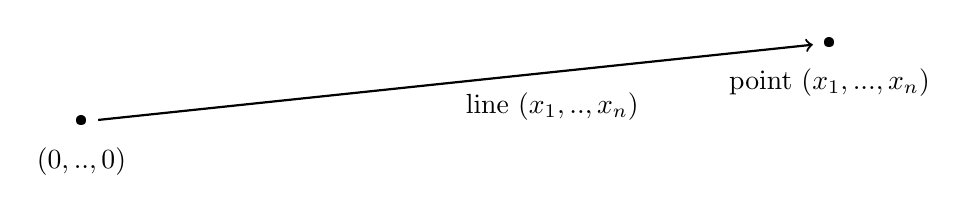
\begin{tikzpicture}[node distance=2cm]
	\node (A)[draw=none,label=below:{$(0,..,0)$}] at (0,0) {\textbullet};
	\node (B)[draw=none,label=below:{point $(x_1,...,x_n)$}] at (9.5,1) {\textbullet};
	
	\draw[thick, ->]
	(A) -- (B) 
	node[midway, below right] {line $(x_1,..,x_n)$};
\end{tikzpicture}

\subsection{Operation with lines}
We need to translate a few more things from euclidean geometry.

\proposition{
Let $\mathbf{x}, \mathbf{y}, \mathbf{z} \in \mathbb{R}^n$, then \[
	\overrightarrow{\mathbf{xy}}+\overrightarrow{\mathbf{yz}}=\overrightarrow{\mathbf{xz}},
\]
where $(a_1,...,a_n)+(b_1,...,b_n)\defeq(a_1+b_1,..., a_n+b_n)$.
}
\begin{proof}
	\begin{align*}
		\overrightarrow{\mathbf{xy}}+\overrightarrow{\mathbf{yz}}&=(y_1-x_1,..., y_1-x_n)+(z_1-y_1,..., z_1-y_n)\\
		&=(y_1-x_1+z_1-y_1, ... ,y_n-x_n+z_n-y_n)\\
		&= (z_1-x_1, ...,z_n-x_n)\\
		&= \overrightarrow{\mathbf{xz}}
	\end{align*}
\end{proof}
\

Geometrically, this means if you connect $\mathbf{x}$ to $\mathbf{y}$ to $\mathbf{z}$, the overall "direction of travel" you make is $\mathbf{x}$ to $\mathbf{z}$. This gives us a natural extension for addition of vectors by considering each entry. Similarly for scaling vectors, we just scale the entries along each dimension.

 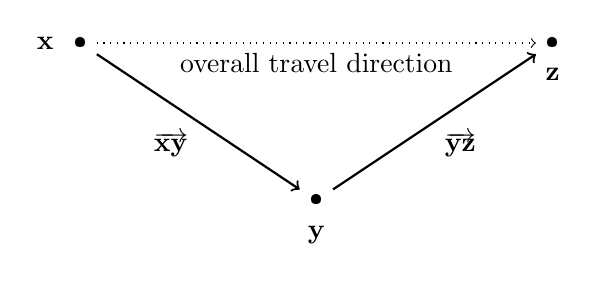
\begin{tikzpicture}[node distance=2cm]
 	\node (A)[draw=none,label=left:$\mathbf{x}$] at (0,0) {\textbullet};
 	\node (B)[draw=none,label=below:$\mathbf{y}$] at (3,-2) {\textbullet};
 	\node (C)[draw=none,label=below:$\mathbf{z}$] at (6,0) {\textbullet};
 
 	\draw[thick, ->]
 	(A) -- (B)
 	node[midway, below left]{$\overrightarrow{\mathbf{xy}}$};
 	\draw[thick, ->]
 	(B) -- (C)
 	node[midway, below right]{$\overrightarrow{\mathbf{yz}}$};
 	
 	\draw[dotted,->]
 	(A)--(C)
 	node[midway, below] {overall travel direction};
 	
 \end{tikzpicture}\ \\

\definition{Addition and scaling of vectors}{
	Let $\vec{a},\vec{b}$ be two vectors in $\mathbb{R}^n$. We define the sum/difference of $\vec{a}$ and $\vec{b}$ \[
		\vec{a}+\vec{b} \defeq (a_1+b_1,...,a_n+b_n), \quad \vec{a}-\vec{b} \defeq (a_1-b_1,...,a_n-b_n)
	\] and the scaling of $\vec{a}$ by a real number $c\in \mathbb{R}$ \[
		c\vec{a} \defeq (c a_1, c a_2,... ,c a_n).
	\]
}
\begin{remark}
	Here we use the term "vectors", as we can in essence add points and lines together. How does one make sense of adding a line to a point? We can view this as translating the point along the path of the line, for instance, let us translate the point $(1,2)$ $3$ units in the first coordinate and $-1$ units in the second coordinate. This will give us $(4,1)$.
 	\textbf{TODO: ADD GRAPH}
\end{remark}
This way, we can write the line from $\vec{x}$ to $\vec{y}$ as $\vec{y}-\vec{x}$. The proof is a computational exercise.
\begin{notation}
	We now transferred for talking about points and the lines between points to addition. Therefore, we can overload the notation for points and lines as a vector $\vec{v}$, keeping in mind that they have the same arithmetic structure.
\end{notation}
\proposition{
	Lines are translation invariant. That is, for every $\vec{x},\vec{y},\vec{v}\in\mathbb{R}^n$, then the 
	line from $\vec{x}$ to $\vec{y}$ is the same as the line from $\vec{x}+\vec{v}$ to $\vec{y}+\vec{v}$.
}
Let us illustrate what this statement is trying to convey. We have two points $\vec{x}$, $\vec{y}$, and now we translate each of these points by $\vec{v}$, and we want the line between the points to be preserved under this translation.
\begin{tikzpicture}
	\node (X)[draw=none,label=left:$\vec{x}$] at (0,0) {\textbullet};
	\node (Y)[draw=none,label=below:$\vec{y}$] at (5,-1) {\textbullet};
	\node (XT)[draw=none,label=below:$\vec{x}+\vec{v}$] at (-2,-2) {\textbullet};
	\node (YT)[draw=none,label=below:$\vec{y}+\vec{v}$] at (3,-3) {\textbullet};
	
	\draw[->,thick] 
	(X)--(Y)
	node (a)[midway, above right] {$\vec{y}-\vec{x}$};
	
	\draw[->,dotted] 
	(X)--(XT)
	node[midway, above left] {$\vec{v}$};
	
	\draw[->,dotted] 
	(Y)--(YT)
	node[midway, above left] {$\vec{v}$};
	
	
	\draw[->,color=blue] 
	(XT)--(YT)
	node[midway, below left] {?};
\end{tikzpicture} \ \\
This statement is easy to verify. In fact, most of our intuition for the real numbers translate to $\mathbb{R}$. For formality, we will list them here; in practice, we (almost always) take these properties for granted.
\proposition{
	Let $\vec{u},\vec{v},\vec{w} \in \mathbb{R}^n$, and $a,b \in \mathbb{R}$. Then the following hold:
	\begin{itemize}
		\item \textit{(Associativity)} $(\vec{u}+\vec{v})+\vec{w} = \vec{u}+(\vec{v}+\vec{w})$.
		\item \textit{(Commutativity)} $\vec{u}+\vec{v} = \vec{v}+\vec{u}$.
		\item \textit{(Identity)} The zero vector $\vec{0}\defeq (0,0,...,0)\in\reals$ satisfies $\vec{v}+\vec{0}=\vec{v}$.
		\item \textit{(Inverse)} The inverse of $\vec{v}$, $-\vec{v}\defeq(-v_1,...,-v_n)$ satisfies $\vec{v}+(-\vec{v})=\vec{0}$.
		\item \textit{(Scalar multiplication)} $a(b\vec{v})=(ab)\vec{v}$.
		\item \textit{(Scalar Identity)} $1\vec{v}=\vec{v}$.
		\item \textit{(Distributivity 1)}  $a(\vec{u}+\vec{v})=a\vec{u}+a\vec{v}$.
		\item \textit{(Distributivity 1)}  $(a+b)\vec{v}=a\vec{v}+b\vec{v}$.
	\end{itemize}
} 
\begin{remark}
	All of these have good geometric intuition behind. For instance, the zero vector $\vec{0}$ is the ``don't move" vector, corresponding to the point at the origin, or the ``too short to be line''. The inverse of $\overrightarrow{\mathbf{xy}}$ is $\overrightarrow{\mathbf{yx}}$, where you go back from $\mathbf{x}$ to $\mathbf{y}$. \begin{tikzpicture}
		
	\end{tikzpicture}
\end{remark}
\begin{remark}
	These $8$ conditions are the axioms of a vector space. Later in the course, we will generalize the notion of vectors in $\reals^n$ to other spaces (playing fields).
\end{remark}
\subsection{Length, angles and projections}
\definition{Magnitude}{
Let $\vec{v}\in\reals^n$. The magnitude of $\vec{v}$ is denoted \[
|\vec{v}| \defeq \sqrt{v_1^2 + v_2 ^2+ ... v_n^2}.
\]
}
We build intuition through the lower dimensional cases.
In $\reals^2$, let us consider the point $(4,3)$.
\begin{wrapfigure}{r}{0.3\textwidth}
	\begin{tikzpicture}
		\node (X)[draw=none,label=left:{$\vec{0}$}] at (0,0) {\textbullet};
		\node (Y)[draw=none,label=left:{$(4,3)$}] at (2,1.5) {\textbullet};
		\draw[->]
		(X)--(Y);
	\end{tikzpicture}
\end{wrapfigure}

The magnitude of this vector is $\sqrt{3^2+4^2}=5$. If this sounds very familiar, it is because this is indeed an application of Pythagorean theorem. In 3-dimensions, this still applies - take $\vec{x}=(a,b,c)$, we can traverse in each coordinate to apply Pythagorean theorem twice.

\usetikzlibrary {3d}

\begin{figure}
	\begin{tikzpicture}
		
		\draw[->](0,0,0) -- (xyz cylindrical cs:radius=3);
		\node at (3.5,0,0){$x_1$};
		\draw[->] (0,0,0) -- (xyz cylindrical cs:radius=3,angle=90);
		\node at (0,3.5,0){$x_2$};
		\draw[->] (0,0,0) -- (xyz cylindrical cs:z=3);
		\node at (0,0,3.5){$x_3$};
		\draw[->,dotted,thick,color=red] (0,0,0) -- (2,0,0);
		\draw[->,dotted,thick,color=red] (2,0,0) -- (2,3,0);
		\draw[->,dotted,thick,color=red] (2,3,0) -- (2,3,1);
		\draw[->,color=blue] 
		(0,0,0) -- (2,3,1)
		node[midway, below]{$\vec{x}$};
	\end{tikzpicture}
	\centering
	\begin{tikzpicture}
		
		\draw[->](0,0,0) -- (xyz cylindrical cs:radius=3);
		\node at (3.5,0,0){$x_1$};
		\draw[->] (0,0,0) -- (xyz cylindrical cs:radius=3,angle=90);
		\node at (0,3.5,0){$x_2$};
		\draw[->] (0,0,0) -- (xyz cylindrical cs:z=3);
		\node at (0,0,3.5){$x_3$};
		\draw[->,dotted,thick,color=red] (0,0,0) -- (2,0,0);
		\draw[->,dotted,thick,color=red] (2,0,0) -- (2,3,0);
		\draw[->,color=brown] 
		(0,0,0) -- (2,3,0)
		node[midway, left]{$\sqrt{a^2+b^2}$};
		
	\end{tikzpicture}
	\begin{tikzpicture}
		[z={(10:10mm)},x={(-45:5mm)}]
		
		\draw[->](0,0,0) -- (3,0,0);
		\node at (3.5,0,0){$x_1$};
		\draw[->] (0,0,0) -- (0,3,0);
		\node at (0,3.5,0){$x_2$};
		\draw[->] (0,0,0) -- (0,0,-3);
		\node at (0,0,-3.5){$x_3$};
		\draw[->,color=brown] 
		(0,0,0) -- (2,3,0)
		node[midway, right]{$\sqrt{a^2+b^2}$};
		
		\draw[->,dotted,thick,color=red] (2,3,0) -- (2,3,-1);
		\draw[->,color=blue] 
		(0,0,0) -- (2,3,-1)
		node[midway, left]{$\sqrt{a^2+b^2+c^2}$};
	
	\end{tikzpicture}
\end{figure}\ \\
To further show this, we can show that multiplying the vector by a number scales the length by exactly that number. 
\proposition{
	Let $\vec{v} \in \reals^n, a\in\reals$. Then \[
	|a\vec{v}| = |a||\vec{v}|.
	\]
}
\example{
Let points A=$(5,8)$, B=$(-2, 7)$, O=$(4,5)$. Find the angle $\angle AOB$.
}
To solve this using only information about the lengths, recall the Law of Cosines:

\theorem{Law of Cosines}{
For any triangle 
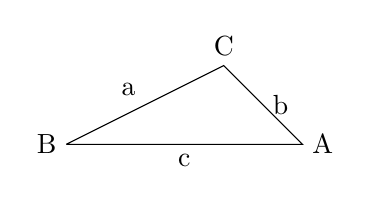
\begin{tikzpicture}
	
	\draw (0,0) node [left] {B}--(2,1) node [above]{C} node [midway, above left]{a}--(3,0) node [right]{A} node [midway, right]{b}--(0,0)node [midway, below]{c};
	%pic["$\alpha$",draw=orange,<->,angle eccentricity=1.2,angle radius=1cm] {angle=(0,0)--(2,1)--(3,0)};
\end{tikzpicture},
\[
	c^2 = a^2+b^2 - 2 a b \cos(\angle BCA).
\]
}

We now apply the Law of Cosines to $\triangle AOB$, so that\[
	|\overrightarrow{AO}|^2  +|\overrightarrow{OB}|^2- 2 |\overrightarrow{AO}| |\overrightarrow{OB} \ |\cos(\angle AOB) = |\overrightarrow{AB}|^2.
\]
Plugging in the values, we solve 
\begin{align*}
		((4-5)^2 + (5-8)^2) + ((-2-4)^2+(7-5)^2) - 2 \sqrt{(4-5)^2 + (5-8)^2} \\ \times \sqrt{(-2-4)^2+(7-5)^2} \cos(\angle AOB) = ((-2-5)^2+(7-8)^2).
\end{align*}
Simplifying, we get\[
	50 - 2 \sqrt{10} \sqrt{40} \cos(\angle AOB) = 50 \implies \cos(\angle AOB) = 0.
\]
So the angle is $\pi/2$.
\exercises
